\section{Unsupervised training and outdoor localization}
\label{subseq:outdoor}
\subsection{Unsupervised depth from monocular training}

\paragraph{Unsupervised depth from monocular at scale.} It is not self-explanatory to claim that the depth maps produced from our unsupervised trained network~\citep{Zhou2017a} are at a real scale. Nevertheless, in our experiment they are because we use the absolute 6-DoF camera pose (obtained by SfM) to compute the relative position and orientation of the training images. In~\citep{Zhou2017a}, authors use an auxiliary relative pose estimation network to make their method trainable with video sequences without any pre-processing. The counterpart is that the final CNN produces depth maps up to an unknown scale factor.

For the case of the Cambridge Landmarks dataset~\citep{Kendall2015}, authors rescale the 3D model obtained by SfM at true scale using control points to obtain meaningful pose error at test time. Some learned depth maps can be found in figure~\ref{fig:depth_map_indoor}, showing that unsupervised method leads to true scale depth values as long as it has been trained with true camera pose information.

\subsection{Comparison with fully-supervised training}
\begin{figure}
    \centering
	\includegraphics[width=\linewidth]{results/indoor/depth_maps}
	\caption[Generated indoor depth maps]{\label{fig:depth_map_indoor} Visualisation of the depth map generated from RGB input with two networks trained with full supervision or without ground truth depth map in an unsupervised manner. In both configurations, networks are trained on the \textbf{7 scenes} dataset~\citep{Shotton2013}. Examples from \textbf{12 scenes}~\citep{Valentin2016} show networks generalisation capability.}
\end{figure}



\subsection{Outdoor localization}
\begin{table}
	\centering
	\begin{scriptsize}
	\begin{tabular}{c l | c c c c c c }
					&	&	Great Court	&	Kings C.	&	Old Hosp.	&	Shop &	St Mary's &	Street \\
		\hline	
	\multirow{2}{*}{{Im. retrieval}}
	& FC-unsup.  	& 27.6/26.79 & 4.4/6.10 & 6.2/10.09 & 4.3/14.93	& 6.9/15.17 & 95.5/58.38 \\
	& C+LSTM-unsup 	& 24.3/20.94 & 5.0/5.86 & 6.5/8.60	& 3.2/9.47  & 5.9/12.71	& 92.5/67.10 \\
	\multirow{2}{*}{{PnlP}}
	& FC-unsup. 	& 25.5/22.64 & 2.9/2.98 & 4.9/6.37 & 1.8/5.78 & 3.5/6.99 & 76.2/51.91 \\
	& C+LSTM-unsup 	& 13.2/10.07 & 2.7/3.10	& 3.5/5.55 & 1.1/3.38 & 2.6/5.85 & 69.5/52.07 \\[1pt]
	\hline
	& {Posenet~\citep{Kendall2017}} & - & 0.9/1.04 & 3.2/3.29 & 0.9/3.78 & 1.6/3.32 & 20.3/25.5 \\
	\end{tabular}
	\end{scriptsize}
	\caption[Pose refinement results on outdoor dataset]{\label{tab:outdoor} Results on the Cambridge Landmarks~\citep{Kendall2015} outdoor dataset, we report median position/orientation error in meters/degree. We compare our two network architectures, FC and C+LSTM, trained in an unsupervised manner.}
\end{table}

As mentioned previously, we only test our unsupervised set-up for outdoor image pose estimation as the Cambridge Landmarks dataset~\citep{Kendall2015} does not contain ground truth depth maps. Results are presented in table~\ref{tab:outdoor}. PnlP performs well on outdoor scene, with a mean improvement of $\times$1.3/$\times$1.4 for FC architecture, and $\times$1.5/$\times$1.6 for C+LSTM, in position/rotation precision over initial pose given by CBIR. Superior performances of C+LSTM model can be explained by a better capability of the recurrent cells in the C+LSTM decoder for modelling the 3D structure of the scene, as shown in figure~\ref{fig:depth_map_outdoor}. Our method is not able to recover a proper pose for the scene Street. As same as for the indoor failure case, this is the result of a poor initial pose estimation at the CBIR preliminary step. Compared to Posenet~\citep{Kendall2017}, our method is marginally less precise but requires only one trained model compared to the 6 models needed by Posenet and can potentially be used on unknown scenes according to the previous indoor experiments. We do not compare our method to Relocnet~\citep{Purkait2018} baseline because authors do not evaluate Relocnet on outdoor scenes.


\begin{landscape}
\begin{figure}
    \centering

	\includegraphics[width=\linewidth]{results/outdoor/depth_maps}
	\caption[Generated outdoor depth maps]{\label{fig:depth_map_outdoor} Visualisation of the depth map generated from RGB input by our two architectures, FC and C+LSTM, trained in an unsupervised manner on Cambridge Landmarks dataset~\citep{Kendall2015}. \textcolor{purple}{Purple boxes} show regions where C+LSTM network produces slightly better depth map reconstruction compared to FC.}
	
\end{figure}
\end{landscape}